\documentclass[12pt]{article}
\usepackage{amsmath}
\usepackage{amssymb}
\usepackage{amsthm}
\usepackage{amsfonts}
\usepackage{graphicx}
\usepackage{textcomp}
\usepackage{hyperref}
\usepackage{tikz}
\usepackage{enumitem}
\usepackage{mathtools}
\usepackage{enumitem}
\usepackage{wasysym}
\usepackage{ulem}
\usepackage{xspace}
\usepackage{csquotes}

\DeclareMathOperator{\dist}{dist}
\DeclareMathOperator{\Nul}{Nul}
\DeclareMathOperator{\Row}{Row}
\DeclareMathOperator{\proj}{proj}

\setlength{\arraycolsep}{12pt}

\newcommand{\defn}{\textbf{Def.}\xspace}
\newcommand{\thm}{\textbf{Thm.}\xspace}
\newcommand{\ex}{\textbf{ex.}\xspace}
\newcommand{\Ex}{\textbf{Ex.}\xspace}
\newcommand{\ie}{\textbf{i.e.}\xspace}
\newcommand{\lemma}{\textit{Lemma}\xspace}
\newcommand{\bproof}{\textit{Proof ($\impliedby$).}\xspace}
\newcommand{\fproof}{\textit{Proof ($\implies$).}\xspace}

\renewcommand{\arraystretch}{1.25} % Adjust row spacing

\hypersetup{
    colorlinks=true,
    linkcolor=blue,
    filecolor=blue,      
    urlcolor=blue,
}

\newcommand{\ulhref}[2]{\href{#1}{\color{blue}\uline{#2}}}

\begin{document}

\title{MACM 316 Lecture 1 - Computer Arithmetic}
\author{Alexander Ng}
\date{Monday, January 6, 2025}

\maketitle

\section{Preface}

Many real-world problems stem from numerical analysis, particularly poor 
execution. Rounding errors, insufficient representation problems, and other 
such problems represent the significant impact of computation in the real world.

Check out the following resources for more information:
\begin{enumerate}
  \item \ulhref{https://www-users.cse.umn.edu/~arnold/disasters/}{https://www-users.cse.umn.edu/~arnold/disasters/}
  \item \ulhref{https://web.ma.utexas.edu/users/arbogast/misc/disasters.html}{https://web.ma.utexas.edu/users/arbogast/misc/disasters.html}
\end{enumerate}

\section{Computer Arithmetic}

We often want to work with the real number system, which consists of all 
integers, rational and irrational numbers

\begin{equation*}
  2, \sqrt{2}, e, \pi, 10^6, \text{ etc.} 
\end{equation*}

Because we have a finite space limitation for numbers, 
\textbf{not all numbers can be represented exactly.} This can cause problems
with arithmetic.

We typically use the decimal (base 10) system, e.g.

\begin{equation*}
  427.325 = 4 \times 10^2 + 2 \times 10^1 + 7 \times 10^{0} + 3 \times 10^{-1}+\dots
\end{equation*}

When we work with a computer, we use the binary (base 2) system, e.g.

\begin{equation*}
  (1001.11101)_2 = 1\times 2^3 + 0\times 2^2 + 0\times 2 + 1\times 2^0 + 1\times 2^{-1} + 1\times 2^{-2} + 1\times 2^{-3} +\dots
\end{equation*}

\section{Error}

Notice that conversion from base-10 to base-2 can lead to errors. It is 
impossible to represent some finite decimal fractions in binary.

\subsection{Example}

Assume $\frac{1}{10} = (0.a_1 \dots a_n)_2$ where $a_i \in \{0, 1\}$.

To convert, we can multiply by 2:

\begin{equation*}
  \frac{2}{10} = 0.2 = (a_1 . a_2 a_3 \dots)_2
\end{equation*}

We take the integer part of both sides:

\begin{align*}
  0.2 &= a_1.a_2 a_3 \dots \\
  0 &= a_1
\end{align*}

Now, we know that $a_1 = 0$. We can continue this process to get the next
digit:

\begin{align*}
  \frac{4}{10} = 0.4 &= a_2.a_3 a_4 \dots \\
  \implies a_2 &= 0 \\
\end{align*}

Again:

\begin{align*}
  \frac{8}{10} = 0.8 &= a_3.a_4 a_5 \dots \\
  \implies a_3 &= 0 \\
\end{align*}

Once more:

\begin{align*}
  \frac{16}{10} = 1.6 &= a_4.a_5 a_6 \dots \\
  \implies a_4 &= 1 \\
\end{align*}

At this point, we know that $a_1 \dots a_3 = 0$ and $a_4 = 1$, all from taking
the integer part of the fraction. Since we just returned a $1$ from this process,
we will subtract $1$ from both sides and continue to the next digit:

\begin{equation*}
  \frac{16}{10} - 1 = \frac{6}{10} = 0.a_5 a_6 \dots
\end{equation*}

Multiply by $2$ to get the next digit:

\begin{align*}
  \frac{12}{10} = 1.2 &= a_5.a_6 a_7\dots \\
  \implies a_5 &= 1
\end{align*}

Again subtract $1$ from both sides:

\begin{equation*}
  \frac{12}{10} - 1 = \frac{2}{10} 
\end{equation*}

Since we got back to $\frac{2}{10}$, which was our starting point, we know that
every part of this process will repeat forever. Therefore, $\frac{1}{10}$ has
an infinitely repeating binary representation. There is \textbf{no} way to 
represent $\frac{1}{10}$ in finite-representation binary.

\begin{equation*}
  \frac{1}{10} = 0.0001100110011\dots
\end{equation*}

\section{Hypothetical Storage Scheme (32-bit)}

We will use a hypothetical decimal computer since the concept is identical.

(By the way, this is almost exactly identical to IEEE-754 floating point
representation, except that we are using a decimal representation instead of
binary.)

Suppose we have the decimal number $423.7$. Since we always want to represent
numbers in \textbf{proper scientific notation}, we normalize the mantissa.

We write our number as follows:

\begin{equation*}
  423.7 = +0.4237 \times 10^{+3}
\end{equation*}

Notice how the $+$ is relevant since we are going to explicitly represent the
sign of the number.

We call the bits following from the decimal point ($4273$) the \textbf{mantissa}.
We include 1 bit for the sign, which is $1$ for positive numbers, 1 bit for the
exponent sign, 7 bits for the exponent, and the remaining 23 bits for the
mantissa. (See diagram below)

\begin{figure}[h]
  \centering
  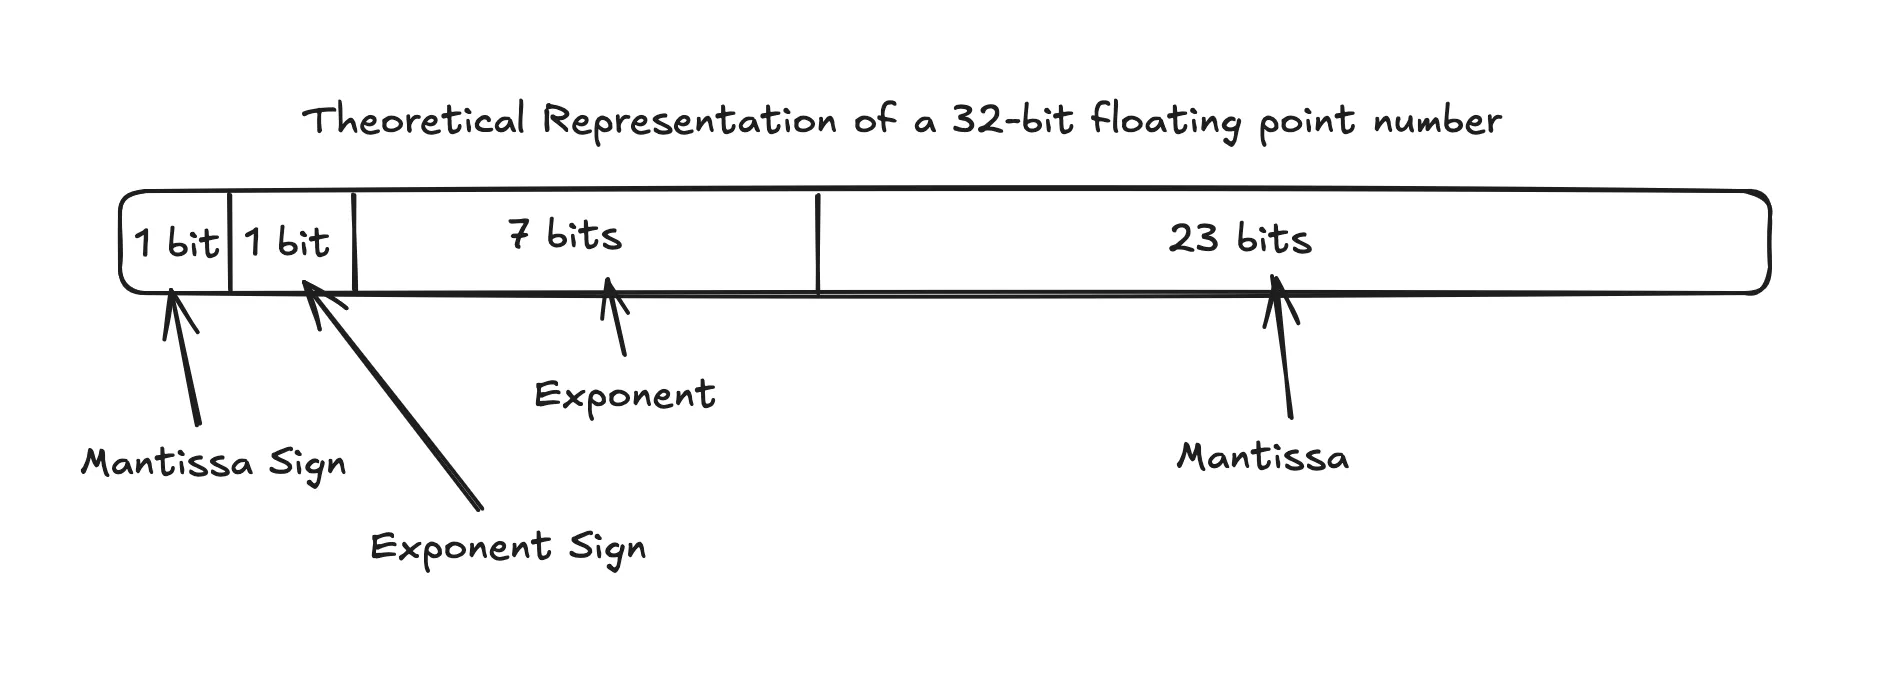
\includegraphics[width=0.8\textwidth]{./fake_ieee754.png}
  \caption{Hypothetical Storage Scheme (32-bit)}
\end{figure}

Because our storage format is finite, one of the biggest problems we will 
encounter is \textbf{bit overflow}. The maximum magnitude of our exponent 
(in binary) is \textbf{127}, so our number can only range from $2^{-127}$ to
$2^{+127}$. Because our mantissa only has 23 bits of precision, the precision
will decrease as our numbers get larger because we use exponentiation to 
represent the actual number.

\Ex:
Consider the number $2^{25} = 33,554,432$. This number can be represented 
exactly in binary. However, the number $2^{25}+1 = 33,554,433$ cannot be
represented exactly, since it can't fit in 23 bits.

All numbers from $2^{25}-1$ through $2^{25}+2$ are represented with the same
mantissa in binary. Only when you reach $2^{25}+3$ does the mantissa change.

Another fun note is that within IEEE-754 floating point representation, the
number of representable values within a given exponent is the same, regardless
of the exponent. This may seem obvious, but it's interesting nonetheless. This
fact comes from the fact that the number of bits in the mantissa is fixed, and
the number of representable values is exactly $2\times 2^{23} = 2^{24}$, since each
positive value has a negative counterpart.

\end{document}
